\documentclass[aspectratio=169, table, 12pt]{beamer}

% Preamble bersama seluruh slide mata kuliah ini.
% Dipanggil dari slides/sessionXX/sessionXX.tex tepat sesudah baris
% \documentclass[aspectratio=169, table, 12pt]{beamer}
% Paket tambahan yang hanya dibutuhkan satu sesi ditulis di berkas sesi itu.

\usepackage{colortbl}
\usepackage{xcolor}
\usepackage{listings}
\usepackage{tabularx}
\usepackage{booktabs}
\usepackage{tikz}
\usepackage{pgfplots}
\pgfplotsset{compat=1.18}
\usetikzlibrary{arrows.meta, positioning, calc, fit, shapes.geometric,
	shapes.multipart, backgrounds, matrix, chains, trees}

\makeatletter
\def\input@path{{../theme/}}
\makeatother
\graphicspath{{../theme/}{../../figures/}}
\usetheme{Pradita}

\definecolor{praditagreen}{RGB}{37, 113, 71}

% Tema membuat garis tabel berwarna putih. Dikembalikan agar tabel terbaca.
\arrayrulecolor{black}
\setlength{\arrayrulewidth}{0.5pt}

\lstdefinelanguage{yaml}{
	basicstyle=\ttfamily\scriptsize,
	keywordstyle=\color{blue}\bfseries,
	commentstyle=\color{gray}\itshape,
	stringstyle=\color{red},
	showstringspaces=false,
	breaklines=true,
	frame=lines,
	numbers=none,
	backgroundcolor=\color{lightgray!10},
	tabsize=2,
	morecomment=[l]{\#}
}

\lstdefinelanguage{json}{
	basicstyle=\ttfamily\scriptsize,
	stringstyle=\color{red},
	commentstyle=\color{gray},
	breaklines=true,
	showstringspaces=false,
	tabsize=2,
	numbers=none,
	frame=lines,
	backgroundcolor=\color{lightgray!10},
	string=[s]{"}{"}
}

\lstdefinelanguage{bash}{
	keywords={},
	basicstyle=\ttfamily\scriptsize,
	ndkeywords={docker, kubectl, helm, curl, git, terraform},
	ndkeywordstyle=\color{purple}\bfseries,
	sensitive=true,
	commentstyle=\color{gray},
	numbers=none,
	breaklines=true,
	frame=lines,
	backgroundcolor=\color{lightgray!10},
	tabsize=2,
	comment=[l]{\#},
	showstringspaces=false
}

\lstdefinelanguage{http}{
	keywords={GET, POST, PUT, PATCH, DELETE, HEAD, OPTIONS, HTTP},
	basicstyle=\ttfamily\scriptsize,
	keywordstyle=\color{blue}\bfseries,
	sensitive=true,
	numbers=none,
	breaklines=true,
	frame=lines,
	backgroundcolor=\color{lightgray!10},
	tabsize=2,
	showstringspaces=false
}

\subtitle{IT40713 · Cloud-Native \& Microservices Architecture}
\author{\textbf{Alfa Yohannis}}


\title{\Huge Resiliensi dan\\ \vspace{10pt} Disaster Recovery}

\begin{document}

\frame{\titlepage}

\begin{frame}
  \frametitle{Isi Pertemuan}
  \vspace{14pt}
  \begin{columns}[t]
    \column{0.5\textwidth}
    {\small\tableofcontents[sections={1-4}]}

    \column{0.5\textwidth}
    {\small\tableofcontents[sections={5-8}]}
  \end{columns}
\end{frame}

\begin{frame}{\hfill}
  \centering
  \Huge{\textbf{Bila satu pusat data\\lumpuh malam ini, layanan\\mana yang harus tetap\\berjalan besok pagi?}}
\end{frame}

\section{Tujuan dan Konteks}

\begin{frame}{\hfill}
  \centering
  \Huge{\textbf{Tujuan dan Konteks}}
\end{frame}

\begin{frame}{{\Large Tujuan Pembelajaran}}
  \vspace{10pt}
  \begin{itemize}
    \item Mengidentifikasi mode kegagalan dalam sistem terdistribusi dan pola resiliensi untuk
          menanganinya.
    \item Menetapkan RTO dan RPO berdasarkan dampak bisnis.
    \item Memilih strategi DR yang seimbang antara biaya dan risiko.
  \end{itemize}
\end{frame}

\begin{frame}{{\Large PDNS 2 Surabaya, Juni 2024}}
  \vspace{6pt}
  \small
  \begin{itemize}
    \item 17 Juni: upaya menonaktifkan Windows Defender terdeteksi; 20 Juni: \textit{ransomware}
          Brain Cipher mulai berjalan.
    \item Tebusan yang diminta 8 juta dolar Amerika Serikat, sekitar Rp131 miliar.
    \item 282 instansi pengguna terdampak; layanan keimigrasian termasuk yang pertama pulih.
    \item Kepala BSSN: hanya 2 persen data di PDNS Surabaya yang memiliki cadangan.
    \item Pelajaran: cadangan yang tidak lengkap atau tidak diuji sama dengan tidak punya cadangan.
  \end{itemize}
  \vspace{4pt}
  {\footnotesize Sumber: ANTARA (27 Juni 2024), CNN Indonesia (26 Juni 2024), CNBC Indonesia
  (28 Juni 2024).}
\end{frame}

\begin{frame}{{\Large Diagram Konsep Bab 12}}
  \centering
  {\small\bfseries Ketahanan request dan pemulihan data saling melengkapi}\par\medskip
  \adjustbox{width=0.96\textwidth,height=0.7\textheight,keepaspectratio}{%
    % Diagram konsep Bab 12: Ketahanan request dan pemulihan data saling melengkapi.
% Dibangkitkan tools/render-diagrams.py dari figures/chapter-diagrams.json;
% ubah data JSON lalu jalankan ulang skrip, jangan sunting berkas ini langsung.
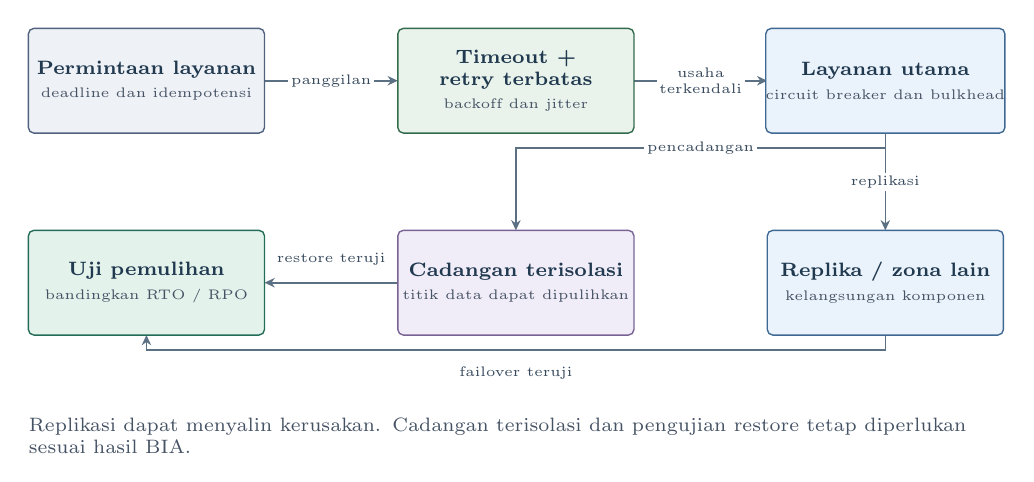
\begin{tikzpicture}[
  x=0.92cm, y=0.95cm,
  kotak konsep/.style={draw, line width=0.5pt, rounded corners=2pt,
    align=center, minimum width=2.999cm,
    minimum height=1.330cm, inner sep=0pt, font=\scriptsize,
    text=konsepJudul},
  peran actor/.style={kotak konsep, fill=konsepIsiActor, draw=konsepGarisActor},
  peran service/.style={kotak konsep, fill=konsepIsiService, draw=konsepGarisService},
  peran control/.style={kotak konsep, fill=konsepIsiControl, draw=konsepGarisControl},
  peran data/.style={kotak konsep, fill=konsepIsiData, draw=konsepGarisData},
  peran outcome/.style={kotak konsep, fill=konsepIsiOutcome, draw=konsepGarisOutcome},
  peran risk/.style={kotak konsep, fill=konsepIsiRisk, draw=konsepGarisRisk},
  panah konsep/.style={-{Stealth[length=1.3mm, width=1.2mm]}, line width=0.6pt,
    draw=konsepPanah},
  panah putus/.style={panah konsep, draw=konsepPanahPutus,
    dash pattern=on 2.5pt off 1.5pt},
  label panah/.style={font=\tiny, align=center, fill=white,
    inner sep=1pt, text=konsepLabel},
  catatan/.style={font=\scriptsize, align=left, anchor=north west,
    inner sep=0pt, text width=12.383cm, text=konsepTeks,
    execute at begin node={\hyphenpenalty=10000\hbadness=10000\relax}},
]
  \definecolor{konsepIsiActor}{HTML}{EEF1F6}
  \definecolor{konsepGarisActor}{HTML}{50627D}
  \definecolor{konsepIsiService}{HTML}{EAF2FB}
  \definecolor{konsepGarisService}{HTML}{3F6893}
  \definecolor{konsepIsiControl}{HTML}{E9F3EC}
  \definecolor{konsepGarisControl}{HTML}{316B4B}
  \definecolor{konsepIsiData}{HTML}{F1EDF8}
  \definecolor{konsepGarisData}{HTML}{786394}
  \definecolor{konsepIsiOutcome}{HTML}{E4F2EC}
  \definecolor{konsepGarisOutcome}{HTML}{236C57}
  \definecolor{konsepIsiRisk}{HTML}{FCEDE7}
  \definecolor{konsepGarisRisk}{HTML}{B36947}
  \definecolor{konsepJudul}{HTML}{20394F}
  \definecolor{konsepTeks}{HTML}{455264}
  \definecolor{konsepLabel}{HTML}{35485C}
  \definecolor{konsepPanah}{HTML}{5C7084}
  \definecolor{konsepPanahPutus}{HTML}{A15D40}
  % Panah dan label lebih dahulu; kotak menutupi sisa latar label.
  \draw[panah konsep] (0.93,0) -- (2.77,0);
  \draw[panah konsep] (6.03,0) -- (7.87,0);
  \draw[panah konsep] (9.5,-0.7) -- (9.5,-2);
  \draw[panah konsep] (9.5,-0.7) -- (9.5,-0.9) -- (4.4,-0.9) -- (4.4,-2);
  \draw[panah konsep] (2.77,-2.7) -- (0.93,-2.7);
  \draw[panah konsep] (9.5,-3.4) -- (9.5,-3.6) -- (-0.7,-3.6) -- (-0.7,-3.4);
  \node[label panah] at (1.85,0) {panggilan};
  \node[label panah] at (6.95,0) {usaha\\terkendali};
  \node[label panah] at (9.5,-1.35) {replikasi};
  \node[label panah] at (6.95,-0.9) {pencadangan};
  \node[label panah] at (1.85,-2.39) {restore teruji};
  \node[label panah] at (4.4,-3.91) {failover teruji};
  \node[peran actor] (request) at (-0.7,0)
    {\textbf{Permintaan layanan}\\[0.5pt]{\tiny\color{konsepTeks}deadline dan idempotensi}};
  \node[peran control] (batas) at (4.4,0)
    {\textbf{Timeout +}\\\textbf{retry terbatas}\\[0.5pt]{\tiny\color{konsepTeks}backoff dan jitter}};
  \node[peran service] (utama) at (9.5,0)
    {\textbf{Layanan utama}\\[0.5pt]{\tiny\color{konsepTeks}circuit breaker dan bulkhead}};
  \node[peran outcome] (pulih) at (-0.7,-2.7)
    {\textbf{Uji pemulihan}\\[0.5pt]{\tiny\color{konsepTeks}bandingkan RTO / RPO}};
  \node[peran data] (backup) at (4.4,-2.7)
    {\textbf{Cadangan terisolasi}\\[0.5pt]{\tiny\color{konsepTeks}titik data dapat dipulihkan}};
  \node[peran service] (replica) at (9.5,-2.7)
    {\textbf{Replika / zona lain}\\[0.5pt]{\tiny\color{konsepTeks}kelangsungan komponen}};
  \node[catatan] at (-2.33,-4.5)
    {Replikasi dapat menyalin kerusakan. Cadangan terisolasi dan pengujian restore tetap diperlukan sesuai hasil BIA.};
\end{tikzpicture}
}
\end{frame}

\begin{frame}{{\Large Resiliensi dan Disaster Recovery}}
  \vspace{10pt}
  \begin{itemize}
    \item Resiliensi: tetap melayani, mungkin dengan fungsi terbatas, ketika sebagian komponen
          gagal.
    \item DR: rencana, arsitektur, dan latihan untuk pulih dari kejadian besar.
    \item IGD tetap menerima pasien pukul tiga dini hari, apa pun yang terjadi pada pusat data.
    \item Pertanyaan dari Bab 1: bagaimana rekam medis dipulihkan bila satu pusat data padam?
  \end{itemize}
\end{frame}

\section{Mode Kegagalan}

\begin{frame}{\hfill}
  \centering
  \Huge{\textbf{Mode Kegagalan}}
\end{frame}

\begin{frame}{{\Large Kegagalan Parsial dan Latensi Tinggi}}
  \vspace{6pt}
  \small
  \begin{itemize}
    \item Sistem terdistribusi jarang gagal total; lebih sering gagal sebagian.
    \item Paling licin: latensi tinggi. Layanan tidak mati, tetapi lambat.
    \item Permintaan yang menunggu $\approx$ laju $\times$ lama menunggu.
    \item 2 per detik $\times$ 0,8 detik $\approx$ 2 menunggu; 2 per detik $\times$ 30 detik =
          60 menunggu.
    \item Kolam 50 koneksi penuh dalam sekitar 25 detik.
  \end{itemize}
  \vspace{4pt}
  {\small Analogi: telepon yang dijawab ``mohon tunggu'' setengah jam lebih merugikan daripada
  telepon yang tidak diangkat.}
\end{frame}

\begin{frame}{{\Large Kegagalan Berantai}}
  \centering
  \eadiagram{../../figures/ch12-kegagalan-berantai.tex}

  \vspace{6pt}
  {\small Titik kegagalan tunggal sering tersembunyi: basis data identitas, sertifikat, satu
  akun, satu orang.}
\end{frame}

\begin{frame}{{\Large Contoh Nyata}}
  \vspace{6pt}
  \small
  \begin{itemize}
    \item AWS US-EAST-1, 7 Desember 2021: lonjakan koneksi membanjiri jaringan internal.
    \item Latensi dan \textit{error} naik, lalu memicu lebih banyak percobaan dan pengulangan.
    \item Kemacetan ikut mengganggu data pemantauan tim operasi.
    \item CrowdStrike, Juli 2024: pembaruan rusak mengenai sekitar 8,5 juta perangkat Windows.
    \item Kurang dari 1 persen mesin Windows, tetapi banyak sektor terdampak pada hari yang sama.
  \end{itemize}
\end{frame}

\begin{frame}{{\Large Enam Mode Kegagalan}}
  \scriptsize
  \begin{tabularx}{\textwidth}{>{\raggedright\arraybackslash}p{3.0cm}
      >{\raggedright\arraybackslash}X >{\raggedright\arraybackslash}p{3.6cm}}
    \hline
    \textbf{Mode} & \textbf{Contoh di Medikara} & \textbf{Pola penanganan} \\
    \hline
    Kegagalan total & Server farmasi RS Depok mati & Salinan ganda, pindah otomatis \\
    \hline
    Latensi tinggi & Cek kepesertaan dari 0,8 menjadi 30 detik & \textit{Timeout},
      \textit{circuit breaker} \\
    \hline
    Kegagalan parsial & Satu dari lima kiriman ke SATUSEHAT ditolak & \textit{Retry} dengan
      \textit{backoff} \\
    \hline
    Kegagalan berantai & Antrean loket memanjang & \textit{Bulkhead}, batas \textit{retry} \\
    \hline
    Titik kegagalan tunggal & Satu basis data identitas & Redundansi, \textit{multi-AZ} \\
    \hline
    Pihak ketiga & Gangguan BPJS Kesehatan, pembaruan vendor & \textit{Graceful degradation} \\
    \hline
  \end{tabularx}
\end{frame}

\begin{frame}{{\Large Kasus Medikara: Gangguan BPJS Merambat ke Loket}}
  \vspace{6pt}
  \small
  \begin{itemize}
    \item Senin 08.10: kepesertaan BPJS Kesehatan melambat dari 0,8 menjadi 30 detik.
    \item Layanan integrasi: 2 permintaan per detik, satu kolam 50 koneksi untuk semua tujuan.
    \item Kolam penuh dalam 25 detik; aplikasi mengulang tiga kali, petugas menekan ``ulangi''.
    \item SATUSEHAT dan pasien umum ikut tertahan.
    \item Pukul 09.30: waktu tunggu loket RS Jakarta naik dari 15 menjadi 70 menit.
  \end{itemize}
  \vspace{4pt}
  {\small Tanpa batas waktu, tanpa sekat, tanpa jalur cadangan.}
\end{frame}

\section{Pola Resiliensi}

\begin{frame}{\hfill}
  \centering
  \Huge{\textbf{Pola Resiliensi}}
\end{frame}

\begin{frame}{{\Large Timeout dan Retry}}
  \vspace{6pt}
  \small
  \begin{itemize}
    \item \textit{Timeout}: batas waktu menunggu; lambat diubah menjadi gagal cepat.
    \item Batas ditetapkan dari data latensi, misalnya persentil ke-99,9 (Brooker).
    \item \textit{Timeout} 3 detik: paling banyak $2 \times 3 = 6$ permintaan menunggu.
    \item \textit{Retry} dengan \textit{backoff} dan \textit{jitter}: jeda makin panjang dan acak.
    \item Bahaya: tiga lapis $\times$ empat percobaan $= 4^3 = 64$ percobaan (buku SRE Google).
  \end{itemize}
  \vspace{4pt}
  {\small Hanya operasi yang aman diulang yang boleh diulang.}
\end{frame}

\begin{frame}{{\Large Circuit Breaker}}
  \centering
  \eadiagram{../../figures/ch12-circuit-breaker.tex}
\end{frame}

\begin{frame}{{\Large Bulkhead dan Graceful Degradation}}
  \vspace{6pt}
  \small
  \begin{itemize}
    \item \textit{Bulkhead}: sekat sumber daya, seperti sekat lambung kapal.
    \item Kolam 50 dibagi: 30 BPJS Kesehatan, 10 SATUSEHAT, 10 tujuan lain.
    \item \textit{Graceful degradation}: fungsi inti tetap jalan dengan mutu diturunkan.
    \item Pasien tetap didaftarkan; kepesertaan ditandai ``periksa ulang''.
    \item Pemeriksaan interaksi obat tidak pernah dilewati, hanya dikerjakan manual oleh apoteker.
  \end{itemize}
\end{frame}

\begin{frame}{{\Large Pendalaman: Simulasi Circuit Breaker}}
  \vspace{6pt}
  \small
  \begin{itemize}
    \item Skrip \texttt{simulasi-circuit-breaker.py}: satu panggilan per detik, gangguan detik 20
          sampai 79.
    \item Tanpa pemutus: 60 gagal setelah menunggu, total tunggu 228 detik.
    \item Dengan pemutus (ambang 5, terbuka 30 detik): 6 gagal, 58 dialihkan, 62,8 detik.
    \item Terbuka detik 24, uji gagal detik 54, tertutup detik 84.
    \item Harga pemutus: 4 permintaan dialihkan walau tujuan sudah sehat sejak detik 80.
  \end{itemize}
\end{frame}

\section{Multi-AZ dan Multi-Region}

\begin{frame}{\hfill}
  \centering
  \Huge{\textbf{Multi-AZ dan Multi-Region}}
\end{frame}

\begin{frame}{{\Large Dua Tingkat Perlindungan}}
  \vspace{6pt}
  \small
  \begin{itemize}
    \item \textit{Multi-AZ}: dua atau tiga zona dalam satu \textit{region}; replikasi sinkron.
    \item \textit{Multi-region}: \textit{region} lain yang jauh; replikasi biasanya asinkron.
    \item Sinkron: tanpa data hilang, tetapi setiap penulisan menunggu lokasi kedua.
    \item Asinkron: cepat, tetapi data yang belum terkirim hilang saat bencana.
    \item AWS: hindari \textit{multi-region} bila \textit{multi-AZ} sudah memenuhi kebutuhan
          bisnis.
  \end{itemize}
  \vspace{4pt}
  {\small Analogi: genset di basement melindungi dari listrik padam, tidak dari banjir.}
\end{frame}

\begin{frame}{{\Large Cakupan Perlindungan untuk Medikara}}
  \centering
  \eadiagram{../../figures/ch12-cakupan-perlindungan.tex}
\end{frame}

\begin{frame}{{\Large Kendala Lokasi Data dan Ukuran Data}}
  \vspace{6pt}
  \small
  \begin{itemize}
    \item Rekam medis ditempatkan di Indonesia (Bab 2); cadangan wajib di tempat berbeda.
    \item Setiap penyedia global hanya punya satu \textit{region} di Indonesia.
    \item Lokasi kedua: penyedia lain, pusat data lokal, atau fasilitas sendiri.
    \item 15 terabyte lewat 1 gigabit per detik: $15 \times 8 \times 10^{12} \div 10^9 =
          120.000$ detik, sekitar 33 jam.
    \item Data besar harus sudah berada di lokasi kedua sebelum bencana.
  \end{itemize}
\end{frame}

\section{RTO, RPO, dan Strategi DR}

\begin{frame}{\hfill}
  \centering
  \Huge{\textbf{RTO, RPO, dan Strategi DR}}
\end{frame}

\begin{frame}{{\Large RTO dan RPO}}
  \centering
  \eadiagram{../../figures/ch12-rto-rpo.tex}

  \vspace{4pt}
  {\small RTO harus lebih pendek dari waktu henti maksimum yang dapat ditoleransi (NIST SP
  800-34).}
\end{frame}

\begin{frame}{{\Large Analisis Dampak Bisnis: Lima Pertanyaan}}
  \vspace{6pt}
  \small
  \begin{enumerate}
    \item Apa yang terjadi bila layanan berhenti 1 jam, 4 jam, dan 24 jam?
    \item Berapa kerugian finansial per jam?
    \item Seberapa besar dampak pada keselamatan pasien?
    \item Kewajiban regulasi atau kontrak apa yang terlanggar?
    \item Berapa waktu henti maksimum yang masih dapat ditoleransi?
  \end{enumerate}
  \vspace{4pt}
  {\small Anggota non-teknis memimpin. Bila biaya pemulihan melebihi biaya kegagalan, strategi
  tidak perlu diterapkan, kecuali ada kewajiban regulasi (AWS).}
\end{frame}

\begin{frame}{{\Large Empat Strategi DR}}
  \centering
  \eadiagram{../../figures/ch12-strategi-dr.tex}
\end{frame}

\begin{frame}{{\Large Kasus Medikara: RTO dan RPO Tiga Layanan}}
  \scriptsize
  \begin{tabularx}{\textwidth}{>{\raggedright\arraybackslash}p{3.4cm}
      >{\raggedright\arraybackslash}X >{\raggedright\arraybackslash}X
      >{\raggedright\arraybackslash}X}
    \hline
    \textbf{Butir} & \textbf{Rekam medis elektronik} & \textbf{Medikara+} &
      \textbf{ERP keuangan} \\
    \hline
    Kerugian per jam & Rp150 juta & Rp40 juta & Rp15 juta \\
    \hline
    Keselamatan pasien & Tinggi & Sedang & Rendah \\
    \hline
    Waktu henti maksimum & 2 jam & 8 jam & 48 jam \\
    \hline
    RTO dan RPO & 1 jam, 5 menit & 4 jam, 15 menit & 24 jam, 60 menit \\
    \hline
    Strategi DR & \textit{Warm standby} & \textit{Pilot light} & \textit{Backup and restore} \\
    \hline
    Biaya DR per tahun & Rp540 juta & Rp120 juta & Rp64 juta \\
    \hline
  \end{tabularx}

  \vspace{8pt}
  \small Total sekitar Rp724 juta per tahun, dibandingkan sekitar Rp3,25 miliar bila semuanya
  \textit{active-active}.
\end{frame}

\section{Ransomware dan Cadangan}

\begin{frame}{\hfill}
  \centering
  \Huge{\textbf{Ransomware dan Cadangan}}
\end{frame}

\begin{frame}{{\Large Replikasi Bukan Cadangan}}
  \vspace{6pt}
  \small
  \begin{itemize}
    \item \textit{Ransomware} berusaha menemukan lalu menghapus atau mengenkripsi cadangan (CISA).
    \item Replikasi menyalin keadaan terkini, termasuk kerusakannya.
    \item Cadangan menyimpan masa lalu, sehingga organisasi dapat kembali.
    \item CISA: cadangan terpisah dari jaringan, terenkripsi, dan diuji berkala.
    \item Penyimpanan yang tidak dapat diubah: salah konfigurasi dapat mahal.
  \end{itemize}
  \vspace{4pt}
  {\small Analogi: salinan akta di brankas bank berkunci waktu, bukan di laci meja kerja.}
\end{frame}

\begin{frame}{{\Large Lima Prinsip Cadangan}}
  \scriptsize
  \begin{tabularx}{\textwidth}{>{\raggedright\arraybackslash}p{2.6cm}
      >{\raggedright\arraybackslash}X >{\raggedright\arraybackslash}X}
    \hline
    \textbf{Prinsip} & \textbf{Artinya} & \textbf{Cara memeriksa} \\
    \hline
    Lengkap & Semua data kritis, konfigurasi, kunci & Dicocokkan dengan daftar layanan kritis \\
    \hline
    Terpisah & Akun, kredensial, jaringan berbeda & Admin produksi gagal menghapus cadangan \\
    \hline
    Tidak dapat diubah & Terkunci selama masa kunci & Percobaan hapus di lingkungan uji ditolak
      \\
    \hline
    Terenkripsi & Tidak terbaca bila dicuri & Kunci disimpan terpisah \\
    \hline
    Teruji & Pemulihan dicoba berkala & Waktu pulih nyata dibandingkan dengan RTO \\
    \hline
  \end{tabularx}

  \vspace{8pt}
  \small Aturan praktis 3-2-1: tiga salinan, dua jenis media, satu di luar lokasi utama.
\end{frame}

\begin{frame}{{\Large Kasus Medikara: Audit Cadangan}}
  \vspace{6pt}
  \small
  \begin{itemize}
    \item 46 aplikasi dalam inventaris Bab 4.
    \item 31 punya jadwal cadangan; 12 pernah diuji pulih dalam 12 bulan terakhir.
    \item Hanya 3 yang cadangannya berada di akun terpisah.
    \item Cadangan SIMRS RS Bandung di server yang sama, dapat dihapus admin domain.
    \item Angka jujur: 3 dari 46 selamat dari \textit{ransomware}.
  \end{itemize}
\end{frame}

\section{Chaos Engineering dan Game Day}

\begin{frame}{\hfill}
  \centering
  \Huge{\textbf{Chaos Engineering\\dan Game Day}}
\end{frame}

\begin{frame}{{\Large Chaos Engineering}}
  \vspace{6pt}
  \small
  \begin{itemize}
    \item Eksperimen untuk membangun keyakinan bahwa sistem tahan kondisi bergejolak.
    \item Empat langkah: keadaan normal terukur, hipotesis, peristiwa nyata, cari selisih.
    \item Cakupan dampak (\textit{blast radius}) ditekan sekecil mungkin.
    \item Netflix: Chaos Monkey mematikan mesin acak pada jam kerja; Chaos Kong sekali sebulan.
    \item Hanya pada sistem sendiri atau yang berizin tertulis; layanan mitra disimulasikan.
  \end{itemize}
\end{frame}

\begin{frame}{{\Large Game Day dan Syarat Aman}}
  \vspace{6pt}
  \small
  \begin{itemize}
    \item \textit{Game day}: latihan terjadwal tim teknis dan bisnis; mulai dari latihan meja.
    \item Medikara: \textit{region} utama tidak tersedia empat jam.
    \item Temuan: layanan identitas hanya di \textit{region} utama; pulih menit ke-80, RTO 1 jam
          meleset.
    \item Syarat: hipotesis terukur, cakupan kecil, kriteria berhenti, izin tertulis.
    \item Pemantauan berjalan dan cara kembali sudah diuji.
  \end{itemize}
\end{frame}

\section{Aktivitas dan Penutup}

\begin{frame}{{\Large Aktivitas: Rencana Resiliensi dan DR}}
  \vspace{6pt}
  \small
  \begin{enumerate}
    \item Ambil dua sampai tiga layanan kritis dari Bab 11 beserta ketergantungannya.
    \item Lakukan analisis dampak bisnis dengan lima pertanyaan.
    \item Tetapkan RTO dan RPO bersama pemilik bisnis.
    \item Pilih strategi DR dan lokasi kedua; perkirakan biaya; petakan pola resiliensi.
    \item Susun skenario uji, jalankan latihan meja, tetapkan jadwal uji setahun.
  \end{enumerate}
\end{frame}

\begin{frame}{{\Large Peran, Luaran, dan Penilaian}}
  \vspace{6pt}
  \small
  \begin{itemize}
    \item Non-teknis: analisis dampak bisnis, kerugian, keselamatan, regulasi.
    \item Teknis: pola resiliensi, strategi DR, lokasi kedua, biaya.
    \item Luaran C4: rencana resiliensi dan DR, skenario uji, jadwal uji pemulihan.
    \item Bobot: dampak bisnis 30, RTO/RPO dan strategi 30, pola 20, skenario uji 20.
    \item Berkas: \texttt{sources/chapter12/} (templat dampak bisnis, rencana DR, skenario).
  \end{itemize}
\end{frame}

\begin{frame}{{\Large Ringkasan}}
  \vspace{6pt}
  \small
  \begin{itemize}
    \item Latensi tinggi dan kegagalan berantai lebih sering daripada kegagalan total.
    \item Lima pola resiliensi; pengulangan harus dibatasi.
    \item \textit{Multi-AZ} untuk satu pusat data; lokasi kedua di Indonesia untuk rekam medis.
    \item RTO dan RPO dari dampak bisnis; strategi termurah yang memenuhi target.
    \item Cadangan terpisah dan tidak dapat diubah; rencana dibuktikan lewat uji terjadwal.
  \end{itemize}
\end{frame}

\begin{frame}{{\Large Latihan}}
  \vspace{6pt}
  \small
  \begin{enumerate}
    \item Jelaskan perbedaan RTO dan RPO dengan contoh layanan rekam medis elektronik.
    \item Pada insiden PDNS 2 tahun 2024, hanya sebagian kecil data yang memiliki cadangan.
          Pelajaran arsitektur dan tata kelola apa yang dapat diambil?
    \item Mengapa strategi \textit{multi-site active-active} belum tentu tepat untuk semua layanan
          Medikara Health?
  \end{enumerate}
\end{frame}

\end{document}
